\documentclass{exam}
\usepackage{xcolor, minted, graphicx, fontspec, siunitx, pgfplots, tabularx}
\setmainfont{Open Sans}
\graphicspath{ {./images} }

\author{Jordy Alkema}
\title {Homework Week 3}

\begin{document}
\maketitle
\section{Review}
\begin{questions}
    \question
    \begin{parts}
        \part
        \textbf{Primary index}
        

        Een index gebasseerd op de primary key waarbij de data geordend als tree wordt opgeslagen. Doordat de primary key unique is en een geordend kan worden wordt de data geordend in de leaf nodes van de tree opgeslagen. Om performanc redenen is het belangrijk dat de primary key klein is.

        \textbf{Secondary index}

        Secondary indexes, ook wel non-primary indexes genoemd zijn indexes die niet unqiue zijn. Ze mogen dus dubbele waardes hebben, zoals een index op een attribute "name". De keys van de nodes zijn hierbij de attribute(s) die zijn geselecteerd(zoals bijv. "name") en de data van de nodes zijn de primary keys. Data opzoeken met behulp van secondary indexes bestaat dus uit twee stappen, de primary key value zoeken via de secondary index en de data row vinden aan de hand van de primary key.

        \textbf{Covering index}
        Een covering index kan alle opgevraagde data van een query vinden zonder verdere lookups te hoeven doen. Stel dat een query id, first\_name en last\_name wil opvragen en een index deze bevat is het niet nodig om verder te zoeken aan de hand van de primary key. Hierdoor is de select query in dit geval erg snel.
        \part
        Bij een clustered index worden de data en indexes op 1 plek opgeslagen. Er is een primary index die de volgorde van de data bepaald(meestal de primary key). De data wordt opgeslagen in een b-tree waar de key van elke node de primary key is en de data de bijbehorende row.


        Een non-clustered index slaat indexes en data apart op. De index beinvloed de volgorde van de data niet. De index wordt puur opgeslagen met een pointer naar de plek waar de data staat. Hierbij staat de data op een andere plek dan de index.
        \part
        De optimizer kijkt naar verschillende variabelen om te kijken hoe de query zo snel mogelijk uitgevoerd kan worden. Zo kijkt ddeze naar welke indexes er gebruikt kunnen worden voor de gemaakte query en welke tables er gebruikt moeten worden. Als er meerdere tables zijn kan het namelijk sneller zijn om te starten met de kleinste table. Ook wordt er bij joins gekeken naar de snelst mogelijke volgorde in het geval van meerdere joins. Soms hoeven bijvoorbeeld niet alle tables compleet uitegelezen te worden maar een beperkt aantal rows aan de hand van de vorige join.
        \part
        De R in R-tree staat voor rectangle. De R-tree is een tree die spatial data efficient kan opslaan door deze op te delen in regios. Elke node in de tree is een regio(rectangle) die in feite het kleinst mogelijke vierkant is waarin alle onderliggende nodes "passen". Elke child node is hierdoor(kwa region) kleiner dan zijn parent node.
        
        Hierdoor is een R-tree erg geschikt voor dit soort queries. De tree is namelijk al gebasseerd op regio's, zo kan er snel worden gezocht in de tree naar de bijpassende regio voor de coordinaten. Hierdoor hoeft niet voor elke row in de database de latitude en longitude te worden bekeken maar kan het zoekdomein beperkt worden tot een veel kleinere regio.

        \part
        Een full-text index is een index die bedoeld is om de zoekprestaties op basis van teksten te versnellen. Een full-text index bevat in plaats van een verwijzing naar de plek van de data de hele tekst. Dit maakt het veel sneller om te zoeken naar bijvoorbeeld een specifiek woord of naar wildcards. Dit maakt het erg geschikt voor het zoeken binnen content die veel tekst bevat zoals documenten of boeken. 
    \end{parts}
\end{questions}

\section{Questions}
\begin{questions}
\setcounter{question}{1}
\question
    \begin{parts}
        \part
        Als er 1000 keys in 1 node kunnen worden opgeslagen zitten er op niveau 4 \(1000^4 = \num{1 000 000 000 000}\) keys. Als elke node 1000 keys kan bevatten zijn er dus \(\num{1 000 000 000 000} / \num{1000} = \num{1 000 000 000}\) leaf nodes aanwezig.
        \part
        Als een B-tree page 16 KB is en een tabelrij 128 bytes groot is kunnen er \(16 KB / 128 bytes = 125\) rijen in een B-tree page worden opgeslagen. Als er \num{1000000000} leaf nodes aanwezig zijn zijn dit dus \(128 * \num{1000000000} = \num{128000000000}\) rijen.
        \part
        Er moeten minimaal 5 B-tree pages worden gelezen waarna 1 write operation moet worden uitgevoerd. Dit zijn dus in totaal 6 i/o operations.
        \part
    \end{parts}
\question
    \begin{parts}
        \part
        Een B-tree is efficient als data geordend kan worden opgeslagen. Deze is dus handig als data in ranges moet worden opgezocht, bijvoorbeeld alle banktransacties in een bepaalde tijdspanne. 

        Hash indexes zijn heel snel maar alleen als er een lookup wordt gedaan die alle elementen van de index bevat. Stel alle banktransacties worden opgeslagen met een naam en transactieid kan de bijbehorende naam van een transactie heel snel gevonden worden door de hash te berekenen van de transactie. Deze rij bevat vervolgens een pointer naar de bijbehorende naam of klant.
        \part
        Hash indexes zijn voornamelijk erg snel om 1 specifieke lookup te kunnen doen, om de bijbehorende voornaam bij bijvoorbeeld een achternaam te vinden zijn ze heel erg snel.
        
        Ook kunnen keys erg groot worden in een B-tree, een hash heeft echter een vaste grootte.
        


        Een hash-index kan echter inefficient worden als er veel hash collisions zijn. Hoe vol een hash table zit kan ook invloed hebben op de performance. Tot slot zijn ze niet geschikt voor het opzoeken van een range aan data zoals bijvoorbeeld ordenen op basis van een specifieke kolom.
        \part
        2, de hash voor 9.876.543 moet worden berekend, als deze berekend is kan direct de bijbehorende record worden gelezen aan de hand van de pointer die in de hash table staat.
    \end{parts}
    \question
    \begin{enumerate}
        \item
            c, een nummer is kleiner(kwa opslag) dan zowel een naam als een code. Aangezien het voor performance het beste is om de primary key zo klein mogelijk te houden is c hier de beste keuze. B kan nuttig zijn als een gebruiker een query moet kunnen schrijven zonder kennis van de database als codes gestandaardiseerd zijn.
        \item
            c, in dit geval is het wederom verstandig om te kiezen voor de kleinste primary key vanwege performance.
        \item
            c, nogmaals is de performance hierbij het beste.
    \end{enumerate}
    \question
    \begin{parts}
        \part
        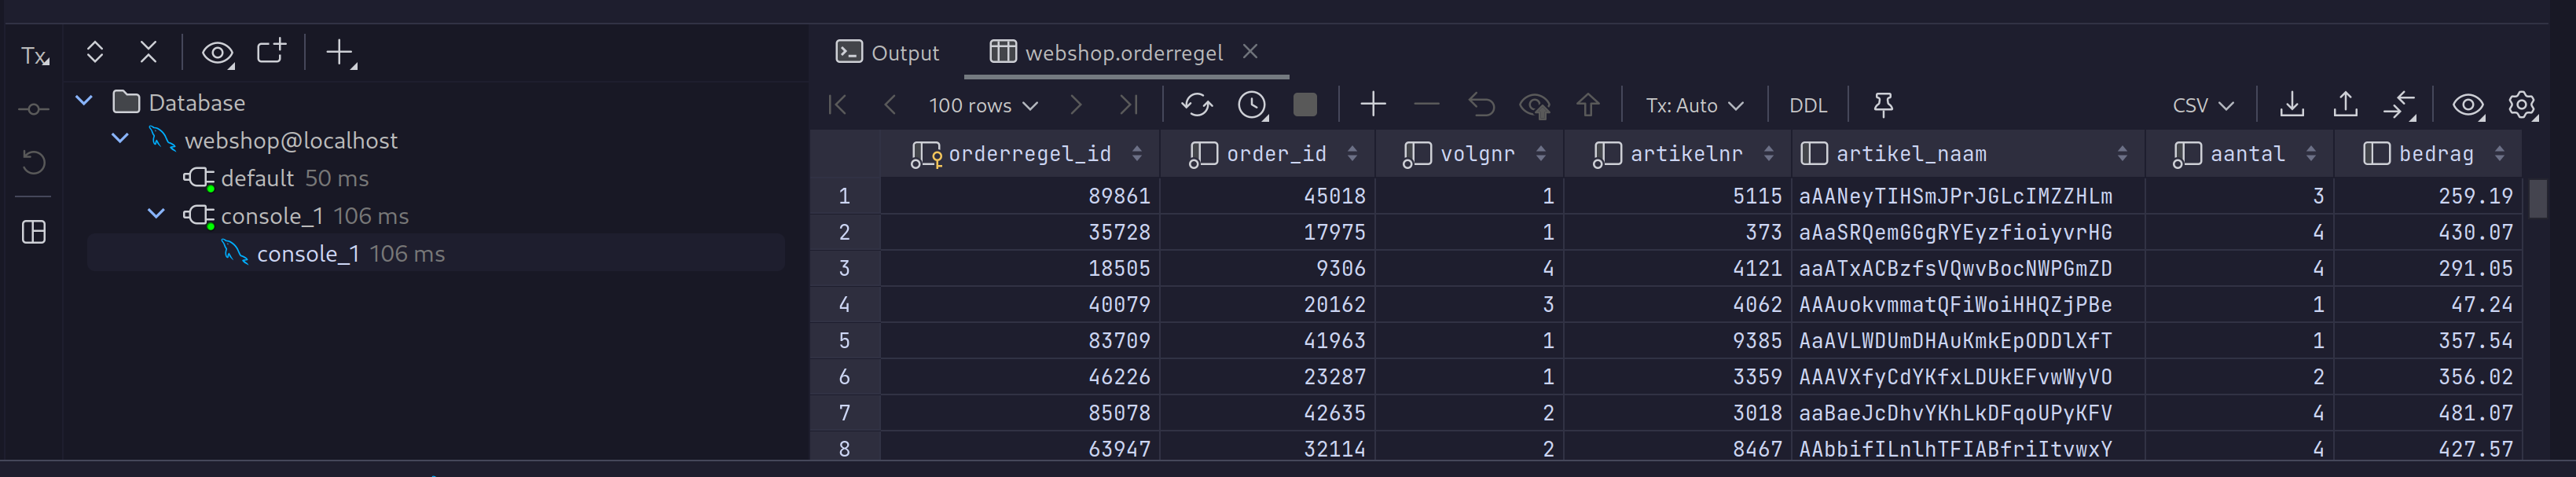
\includegraphics[height=\textheight, width=\textwidth, keepaspectratio]{question5a}
        \part
        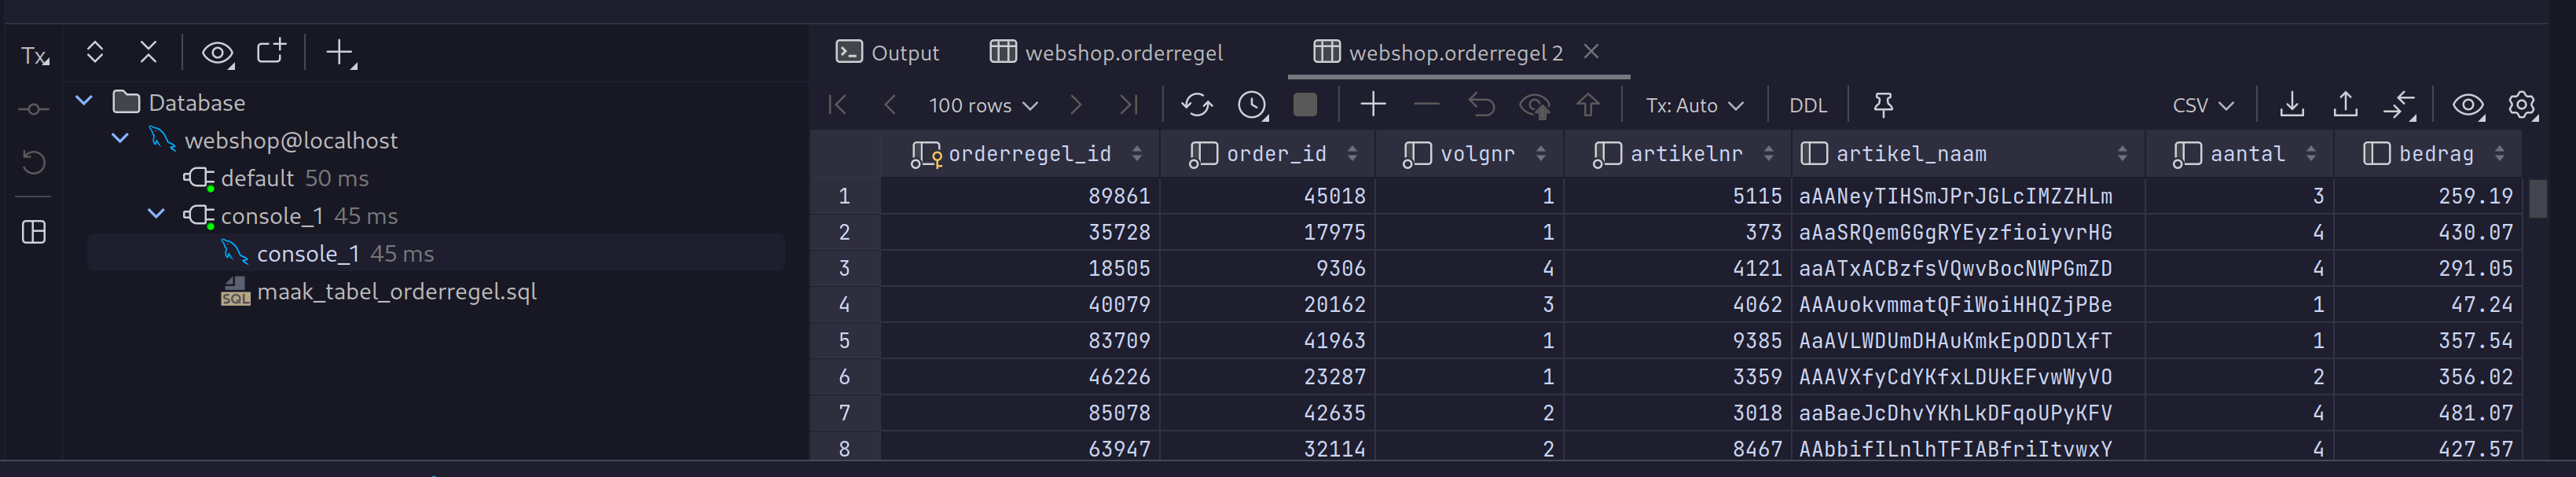
\includegraphics[height=\textheight, width=\textwidth, keepaspectratio]{question5b}

        Bij a moet de hele tabel langs gegaan worden aangezien deze standaard geordend wordt op de primary key. Voor alfabetisch sorteren moet daarom elke row worden bekeken waarna hij pas geordend kan worden. Een index aanmaken op artikel\_naam zorgt ervoor dat er ook op volgorde van artikel\_naam wordt opgeslagen in een secondary index. Als er gevraagd wordt om een sortering op basis van artikel naam gebruikt de optimizer hier deze index voor en hoeft hij alleen door de tree heen te gaan en met behulp van de primary keys de gevraagde columns opvragen. Hierdoor hoeft dus niet meer de hele tabel van 100k rows eerst gelezen te worden.
        \part
        \begin{tabular}{ |c|c|c|c|c|c|c|c|c|c|c| }
            \hline
            n & 0 & 50 & 100 & 150 & 200 & 250 & 300 & 350 & 400 & 450 \\
            \hline
            zonder index & 59 & 66 & 64 & 70 & 66 & 81 & 67 & 58 & 61 & 70 \\
            \hline
            met index & 45 & 53 & 50 & 50 & 47 & 54 & 41 & 45 & 39 & 45 \\
            \hline
        \end{tabular}
        \part
        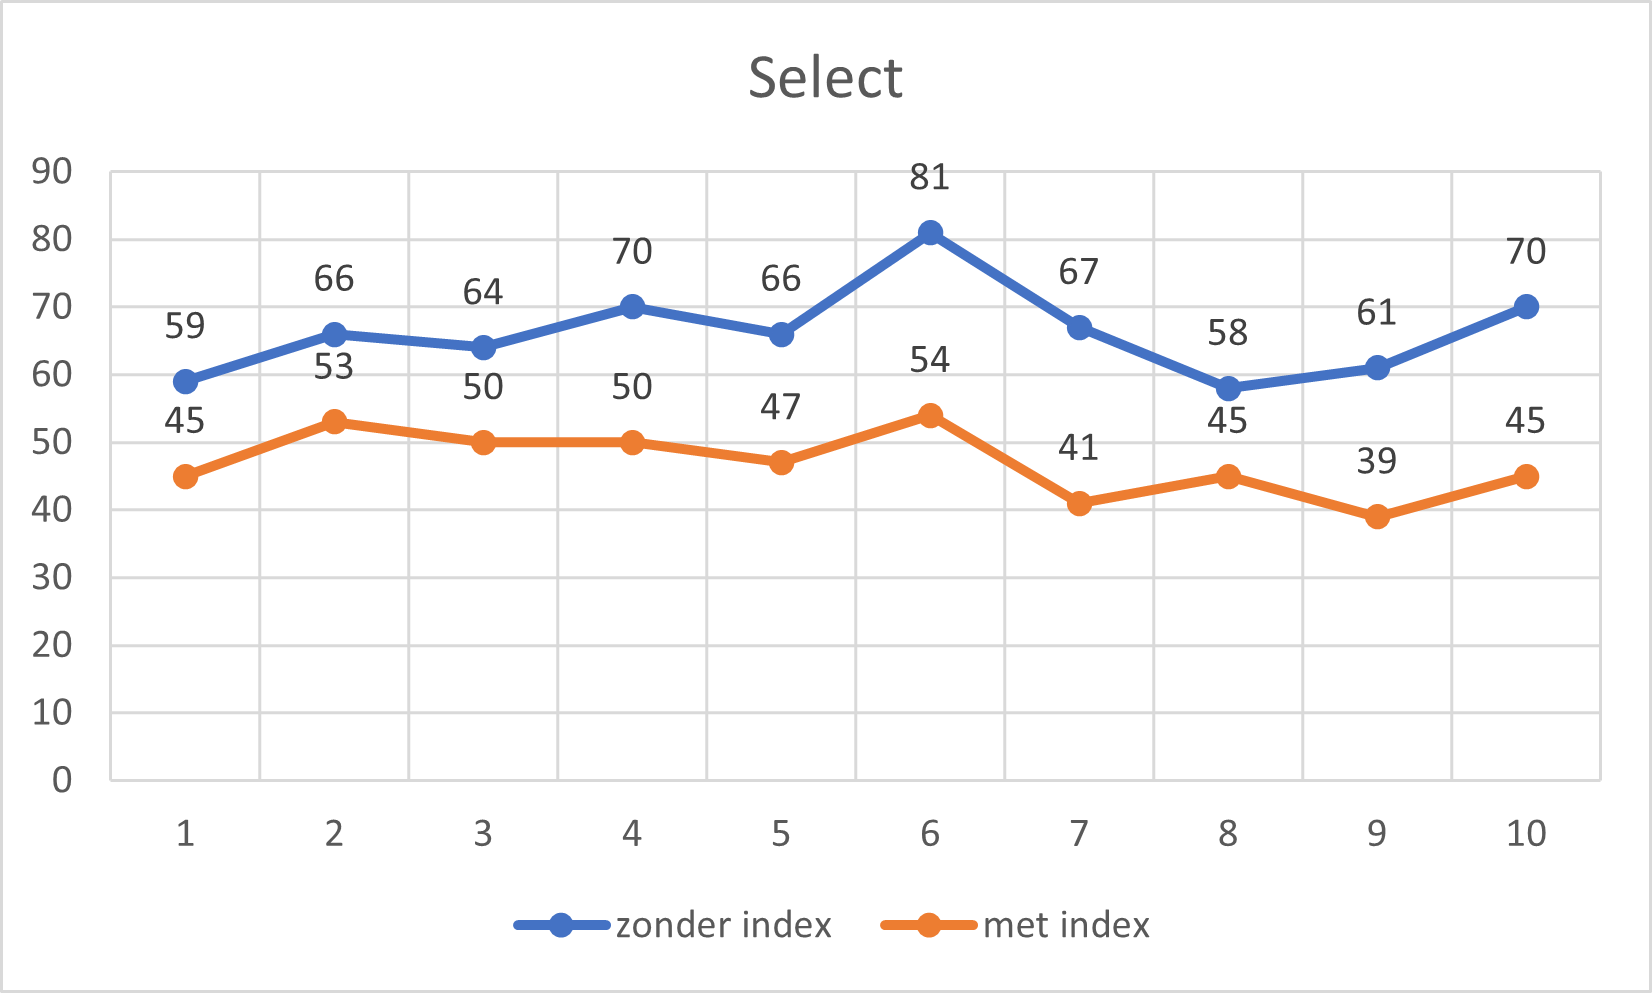
\includegraphics[height=\textheight, width=\textwidth, keepaspectratio]{question5d.png}
        In het verloop lijkt in beide grafieken weinig logica te zitten. Met index is de tijd die nodig is consistent korter. Dit valt te verklaren doordat deze index alle data representeert als een b-tree geordend op basis van de prijs. Om te kijken naar een bepaalde prijs range hoeft dus niet de hele tabel lansgegaan te worden. Er hoeft alleen in de tree gekeken te worden naar de bedragen en aan de hand hiervan kunnen met de primary key de bijbehorende waardes geselecteerd worden.
    \end{parts}
    \question
    \begin{parts}
        \part
        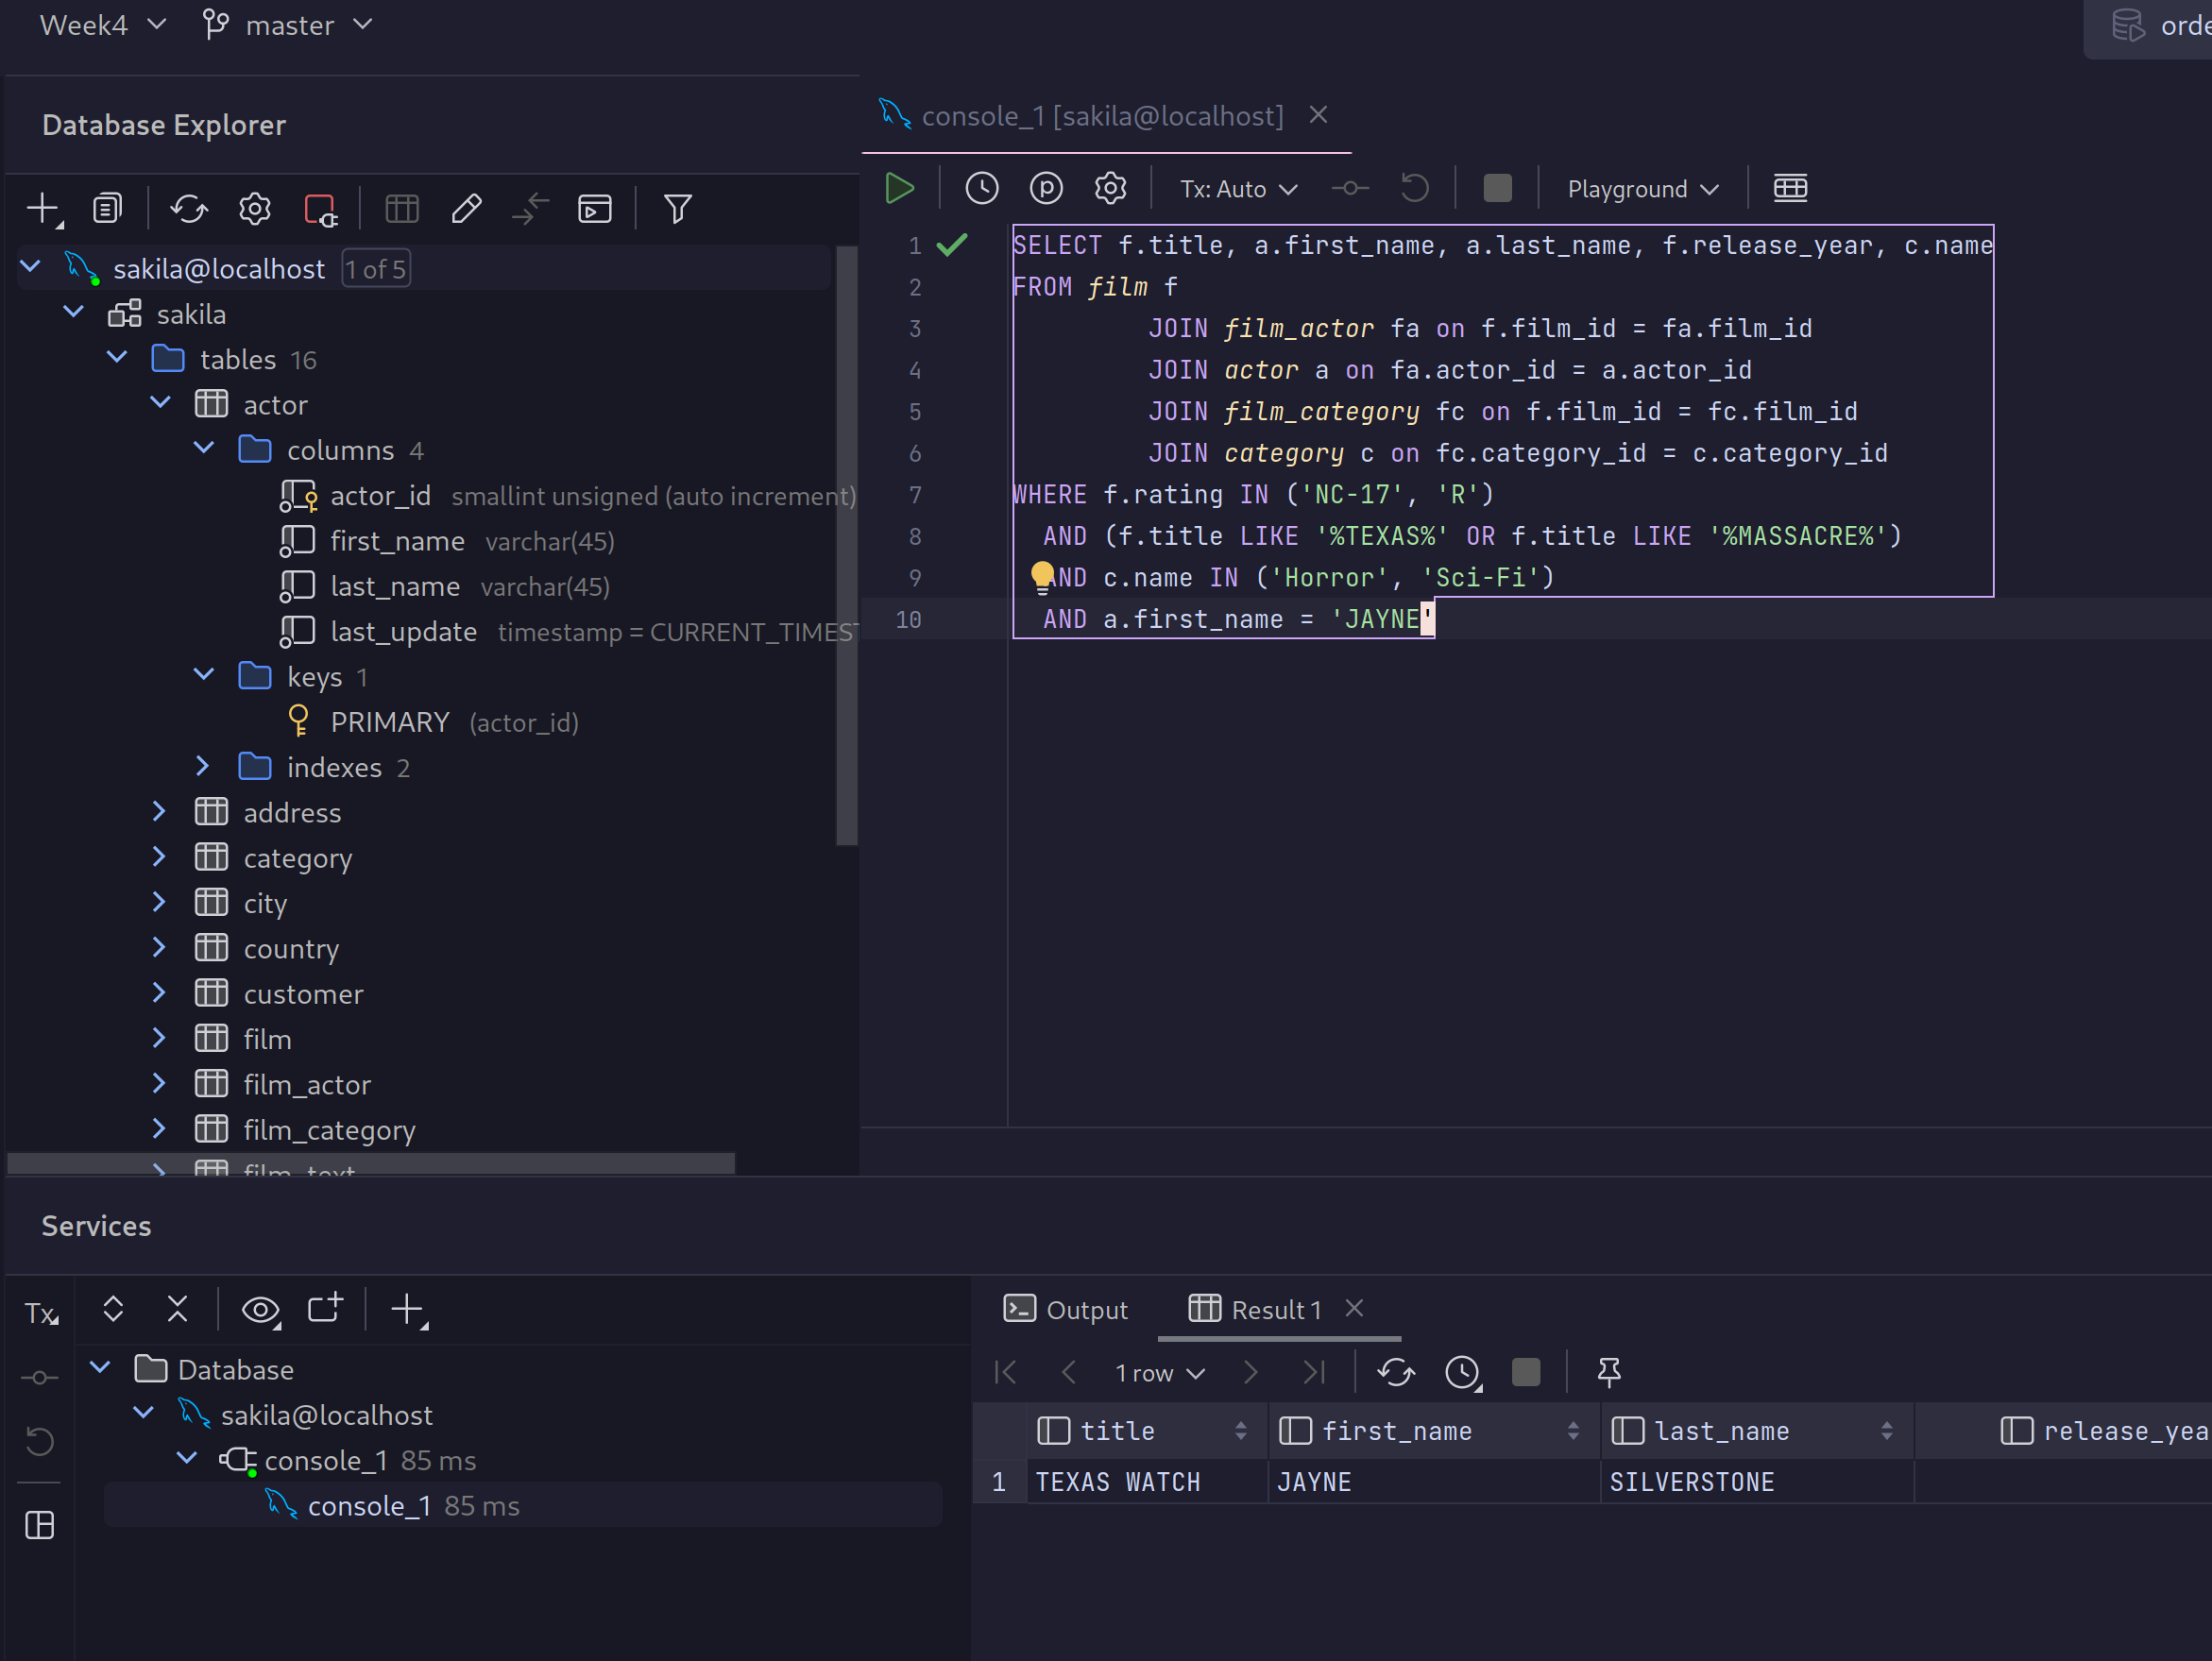
\includegraphics[height=\textheight, width=\textwidth, keepaspectratio]{question6a}
        \part
        65535
        \part
        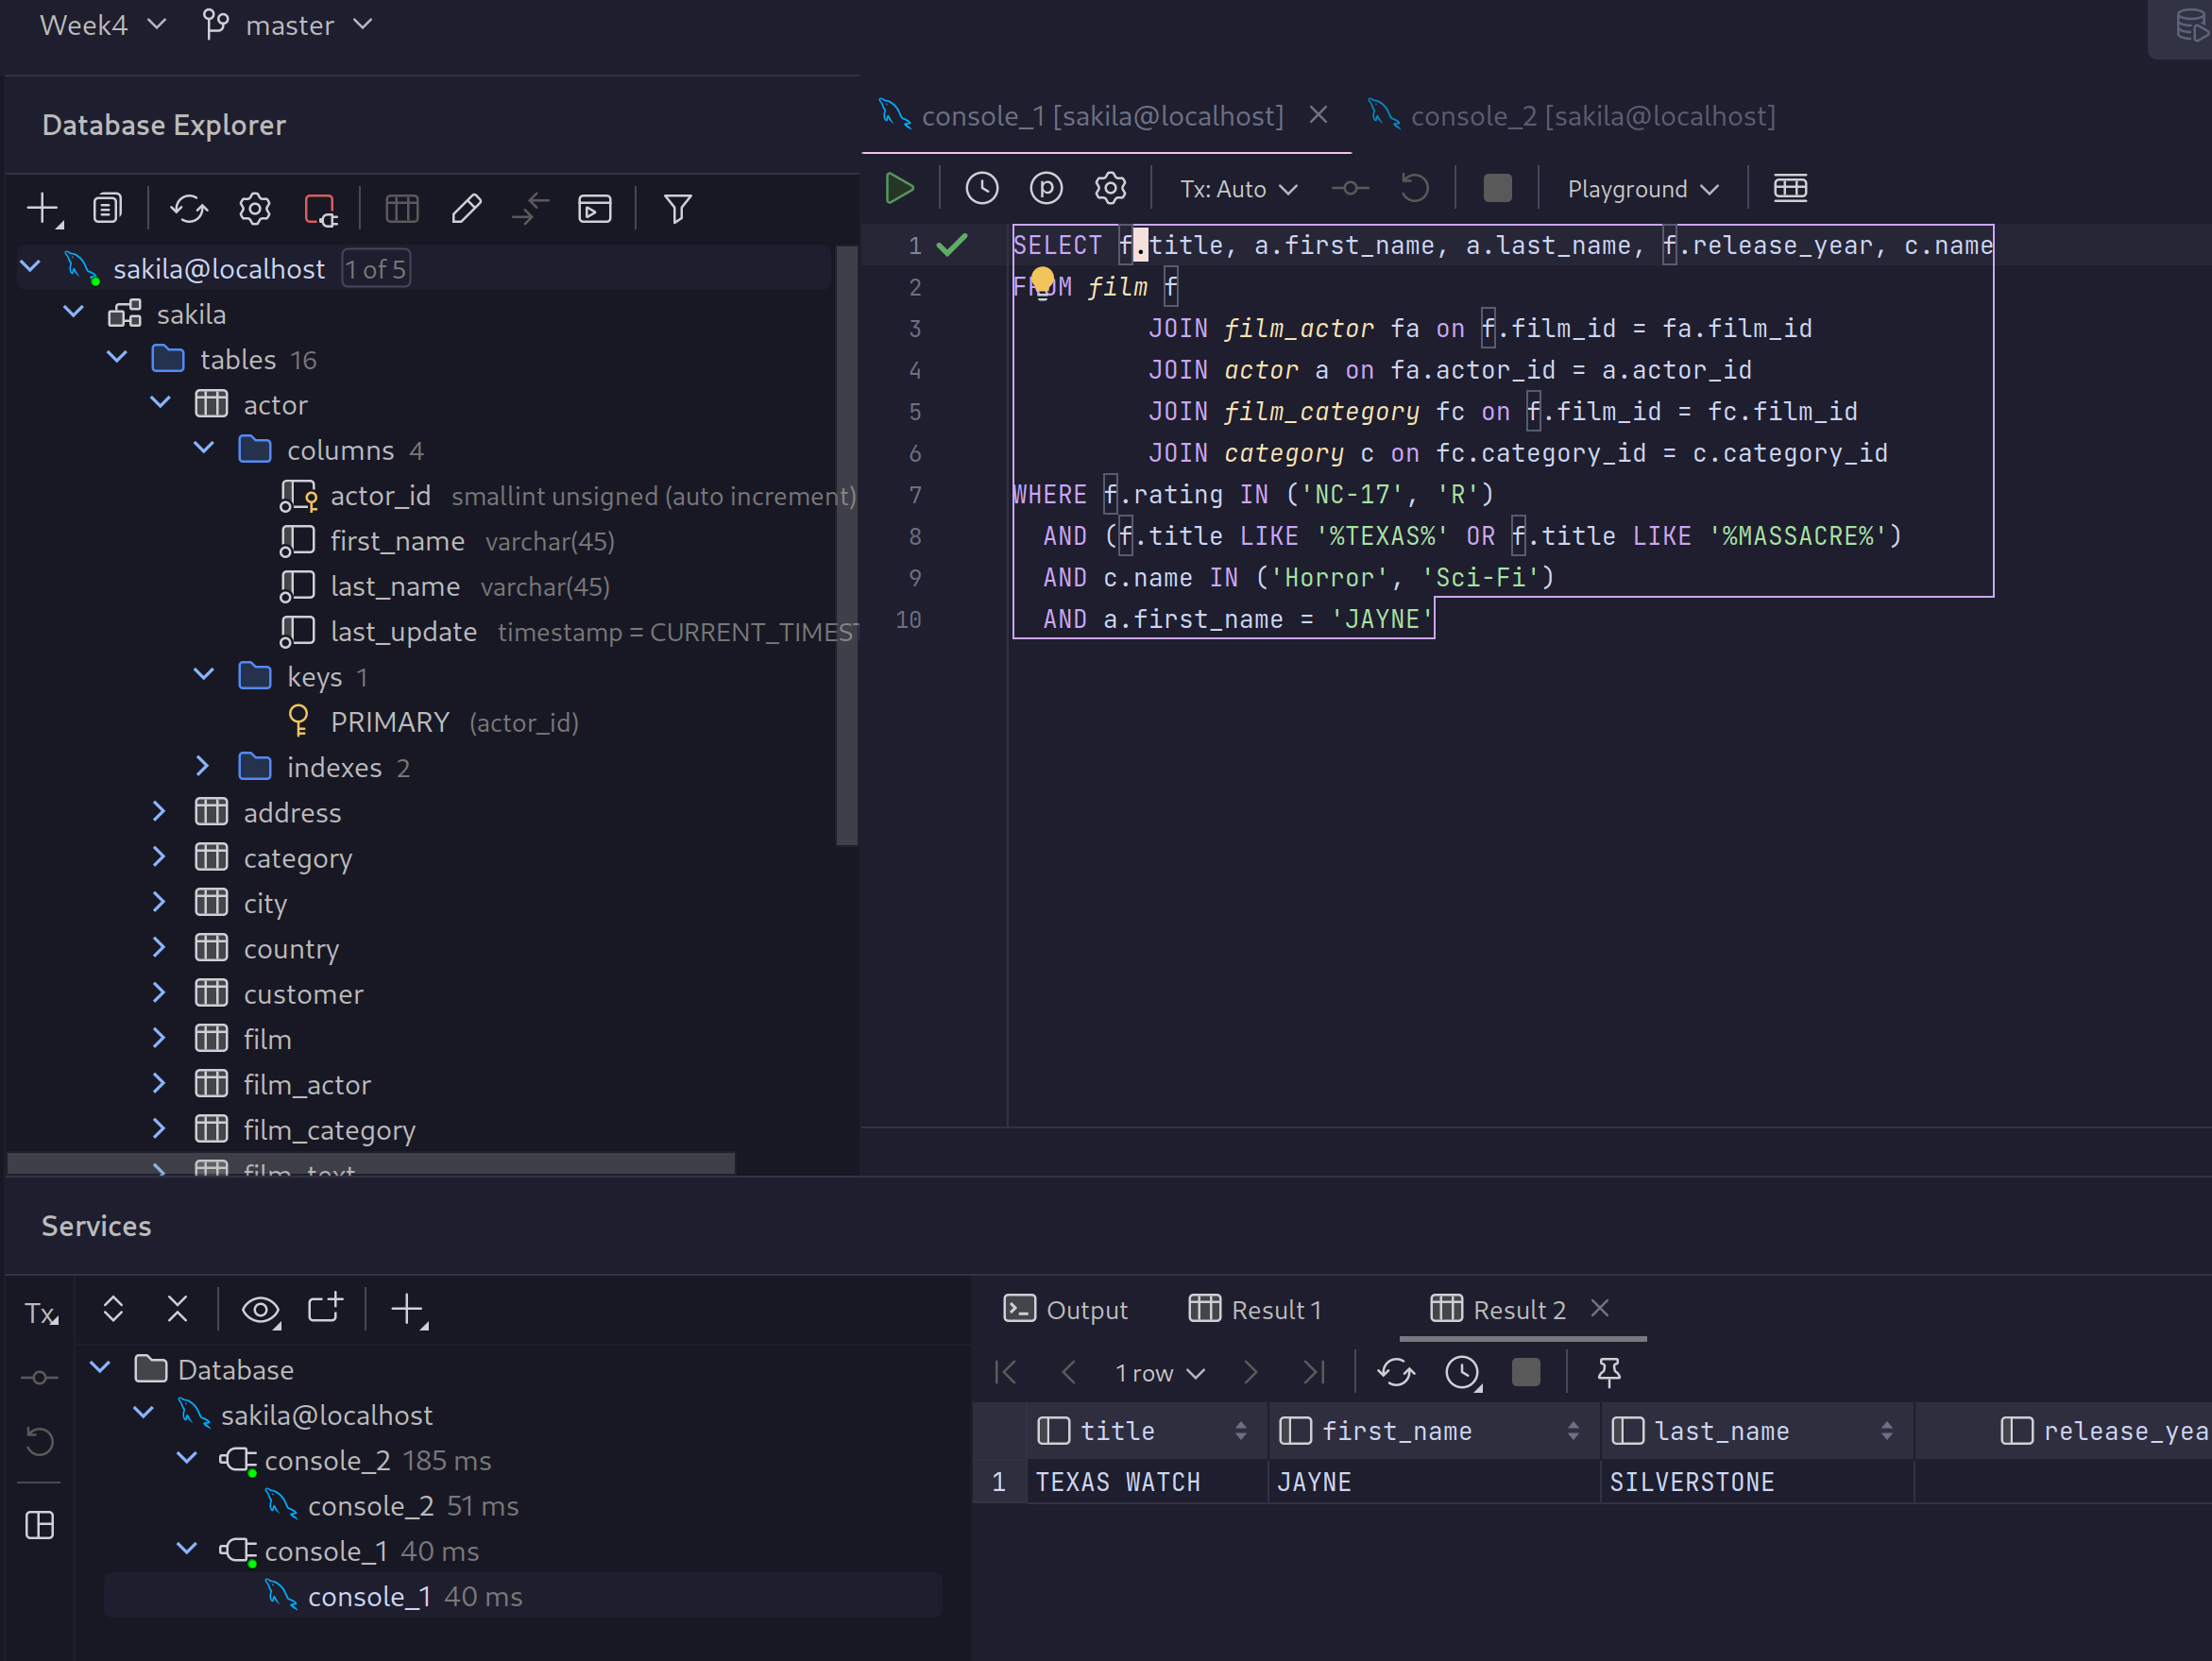
\includegraphics[height=\textheight, width=\textwidth, keepaspectratio]{question6c}
        \part
        Omdat het result gecached wordt, aangezien er indexes aanwezig zijn kan door de analyze commands worden gecheckt of de nieuwe rows de query beinvloeden.
        \part
        \begin{enumerate}
            \item
            Welke producttabel?
            \item
                \begin{tabular}{|p{2cm}|p{2cm}|p{2cm}|p{2cm}|p{2cm}|p{2cm}|}
                    \hline
                    tabel & category & film\_category & film & film\_actor & actor \\
                    \hline
                    aantal rijen & 375 & 375 & 1 & 1 & 1 \\
                    \hline
                    gebruikte key & & & & & \\
                \end{tabular}
                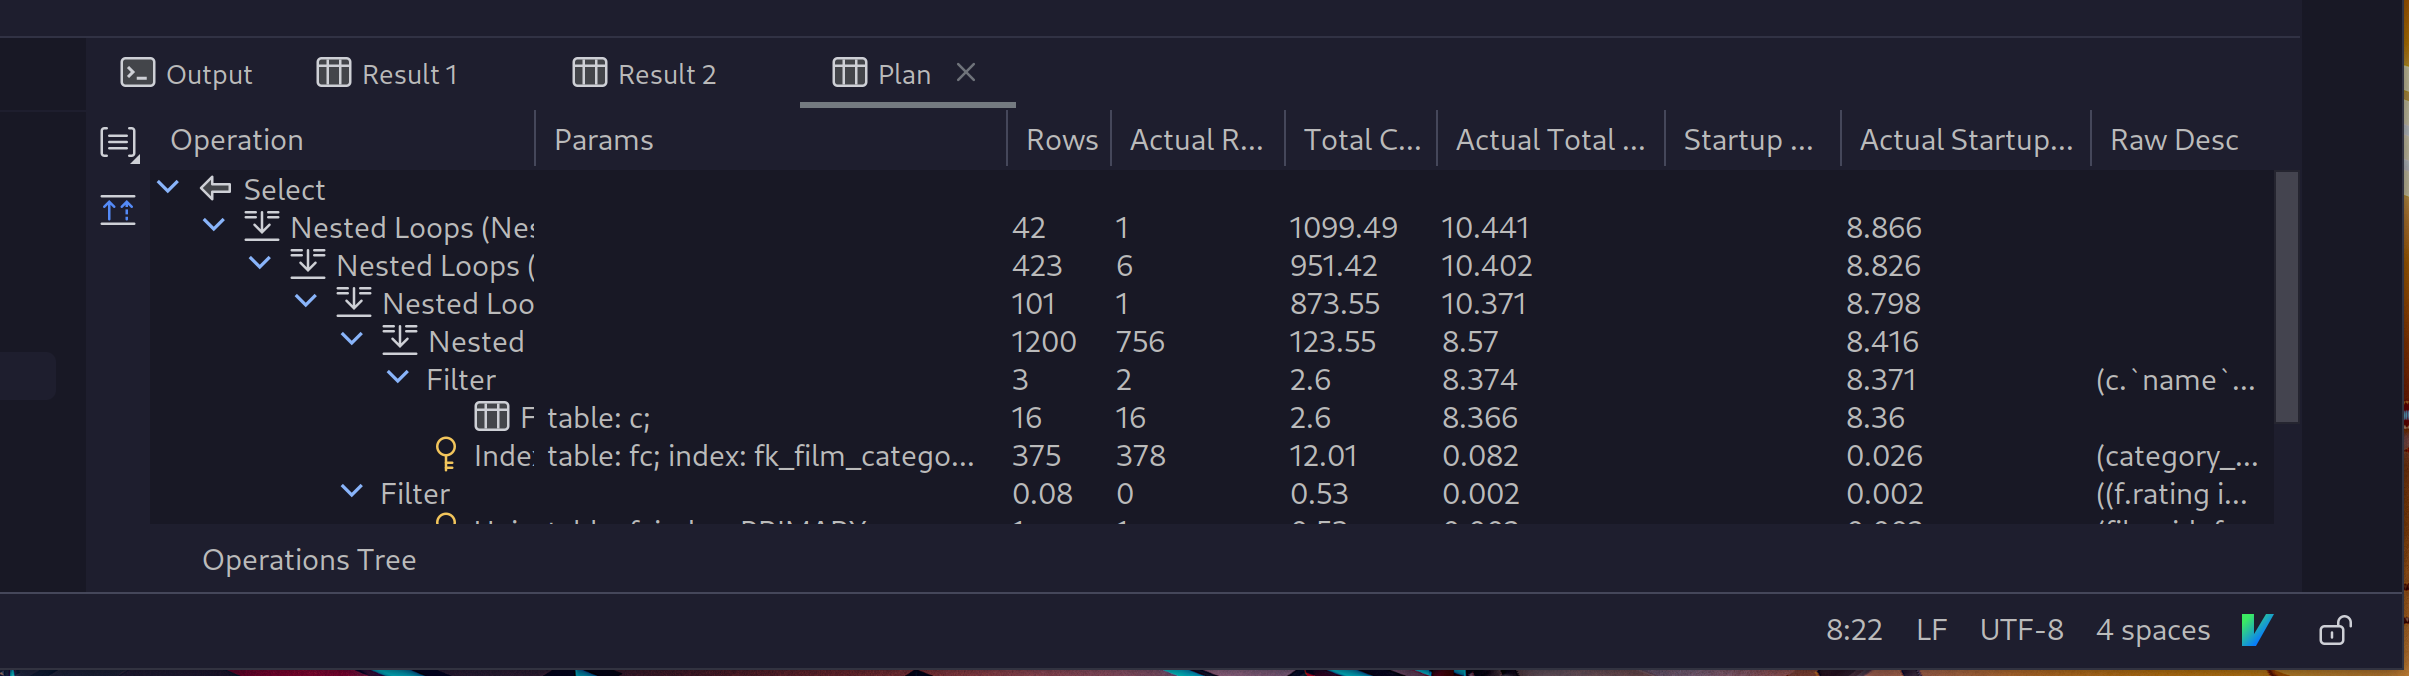
\includegraphics[height=\textheight, width=\textwidth, keepaspectratio]{question6d}
        \end{enumerate}
        \part
        \part
        Een index op actor.first\_name, category\_name, scheelt ongeveer 20 ms


        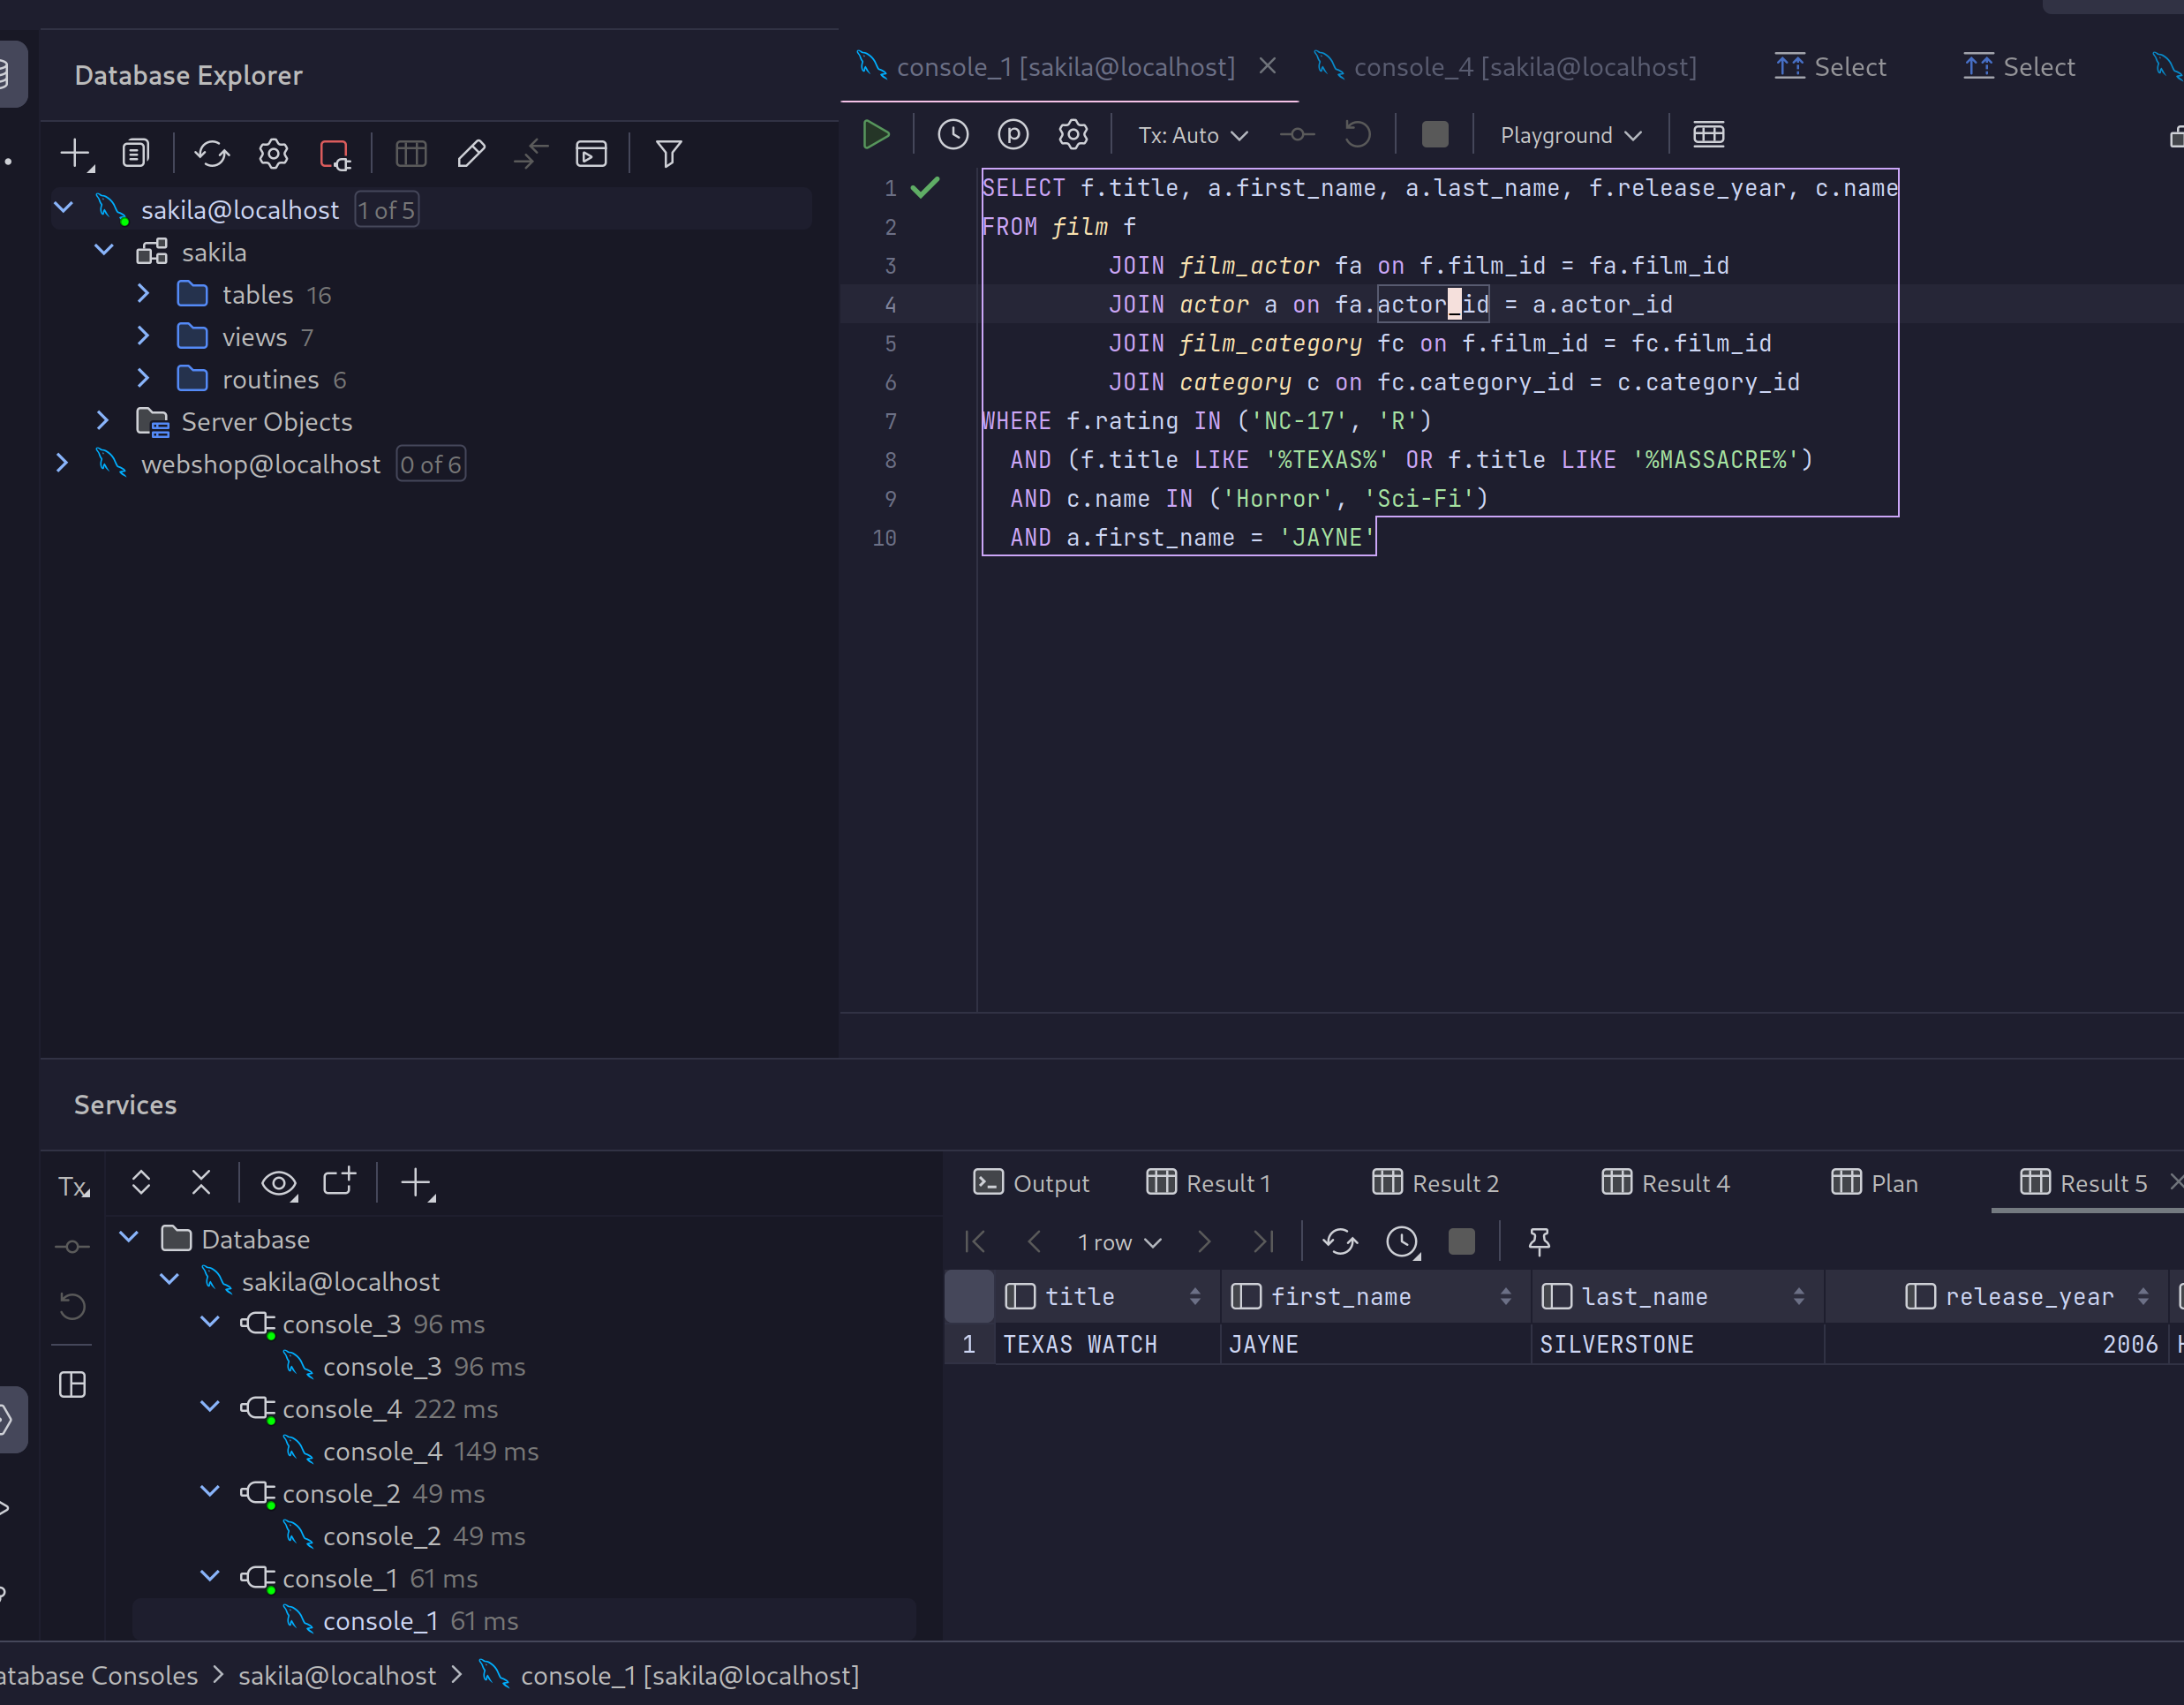
\includegraphics[height=\textheight, width=\textwidth, keepaspectratio]{question6e}
    \end{parts}
\end{questions}
\end{document}
